\ifdefined\standalone
\documentclass[12pt]{article}
\usepackage{graphicx}
\usepackage{float}
\usepackage[a4paper, margin=1in]{geometry}
\usepackage[utf8]{inputenc}
\usepackage{textcomp}
\usepackage{amsmath}
\usepackage[hidelinks]{hyperref}
\usepackage{tikz}
\usetikzlibrary{decorations.pathmorphing,patterns}
\begin{document}
\fi

\section{Convective Cooling}

This case investigates one-dimensional transient heat conduction in a thick slab of thickness $L = 1~\mathrm{m}$. 
The slab is initially at a uniform temperature of $T_{ini} = 1000~^\circ\mathrm{C}$ and is exposed to ambient air at 
$T_\infty = 0~^\circ\mathrm{C}$ on one face. Heat exchange at the exposed surface occurs by convection and is characterized 
by a heat transfer coefficient $h_c = 1~\mathrm{W\,m^{-2}\,K^{-1}}$. 
The opposite face is assumed to be perfectly insulated. 
The configuration is illustrated in Figure~\ref{fig:heat_conduction_configuration}. 
The thermophysical properties of the slab material are summarized in Table~\ref{tab:thermal_properties_heat_conduction}.

The numerical results are presented in Figure~\ref{fig:heat_conduction_results} and are compared with the analytical solution 
reported by Incropera et al.~\cite{incropera_fundamentals_2007}, which follows the same formulation as 
Equation~\ref{Eq:Thermal_thranscendantale}.

\begin{table}[H]
\centering
\caption{Thermophysical properties of the slab material.}
\label{tab:thermal_properties_heat_conduction}
\renewcommand{\arraystretch}{1.3}
\begin{tabular}{c c c}
\hline
$k$ ($\mathrm{W\,m^{-1}\,K^{-1}}$) &
$c_p$ ($\mathrm{J\,kg^{-1}\,K^{-1}}$) &
$\rho$ ($\mathrm{kg\,m^{-3}}$) \\
\hline
1 & 1 & 1000 \\
\hline
\end{tabular}
\end{table}

\begin{figure}[H]
\centering
\begin{minipage}[t]{0.48\textwidth}
\centering
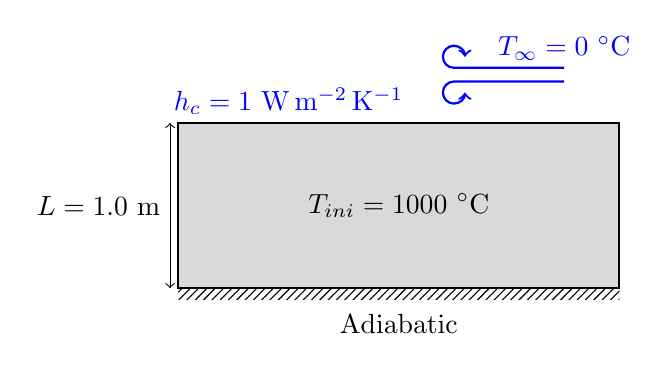
\begin{tikzpicture}[scale=0.7]

\draw[fill=gray!30,thick] (0,0) rectangle (8,3); 
\node at (4,1.5) {$T_{ini} = 1000~^\circ\mathrm{C}$};

\draw[<->] (-0.15,0) -- (-0.15,3);
\node[left] at (-0.15,1.5) {$L=1.0~\mathrm{m}$};

\draw[->,thick, blue] (7,3.75) -- (5,3.75) 
arc[start angle=90, end angle=360, radius=0.2cm]; 
\draw[->,thick, blue] (7,4) -- (5,4) 
arc[start angle=270, end angle=0, radius=0.2cm]; 

\node[blue] at (2,3.4) {$h_c = 1~\mathrm{W\,m^{-2}\,K^{-1}}$};
\node[blue] at (7,4.35) {$T_\infty = 0~^\circ\mathrm{C}$};

\fill[pattern=north east lines] (0,-0.2) rectangle (8,0);
\node[below] at (4,-0.3) {Adiabatic};

\end{tikzpicture}
\caption{Schematic representation of the heat conduction configuration.}
\label{fig:heat_conduction_configuration}
\end{minipage}
\hfill
\begin{minipage}[t]{0.48\textwidth}
\centering
\includegraphics[width=\textwidth]{convective_cooling.png}
\caption{Temporal evolution of temperature at different locations within the solid.}
\label{fig:heat_conduction_results}
\end{minipage}
\end{figure}


\ifdefined\standalone
\end{document}
\fi
